\chapter{PVA Scaffold Engineering for PCM Confinement}\label{ch:pva}

\section{Molecular Structure and Hydrogen Bonding}
Polyvinyl alcohol consists of repeating $[-CH_2-CHOH-]_n$ units enabling extensive hydrogen bonding. The hydrogen-bond density proxy is
\begin{equation}\label{eq:hb_density}
\chi_{HB}=\frac{N_{OH}^{eff}}{V},
\end{equation}
which correlates with modulus and water sensitivity.

\section{Crystallinity and Mechanical Properties}
The crystallinity index from XRD deconvolution can be represented as
\begin{equation}\label{eq:crystallinity}
X_c=\frac{A_c}{A_c+A_a}.
\end{equation}
A rule-of-mixtures estimate for elastic modulus under porosity is
\begin{equation}\label{eq:modulus_porosity}
E_{eff}=E_0(1-\phi_p)^n,
\end{equation}
where $\phi_p$ is porosity and $n$ captures microstructure morphology.

\section{Freeze-Drying and Hierarchical Porosity}
Directional freezing and lyophilization generate micro-to-nano pores. Permeability scales as
\begin{equation}\label{eq:kozeny}
K\sim\frac{\phi_p^3}{(1-\phi_p)^2 S_v^2},
\end{equation}
with $S_v$ the specific surface area.

\section{PCM Confinement Physics}
Capillary pressure in pores is
\begin{equation}\label{eq:capillary}
\Delta p_c=\frac{2\gamma\cos\theta}{r_p},
\end{equation}
which promotes leakage resistance when pore radii $r_p$ are sufficiently small. Effective retained PCM fraction is
\begin{equation}\label{eq:retention}
\Phi_{ret}=1-\exp\left(-\alpha\frac{\Delta p_c}{\rho g h}\right).
\end{equation}

\section{Mechanical Stability under Cycling}
Damage accumulation can be represented by
\begin{equation}\label{eq:damage}
D_N=1-\left(\frac{\sigma_f(N)}{\sigma_f(0)}\right),
\end{equation}
where lower $D_N$ indicates stable scaffold mechanics.

\begin{figure}[htbp]
\centering
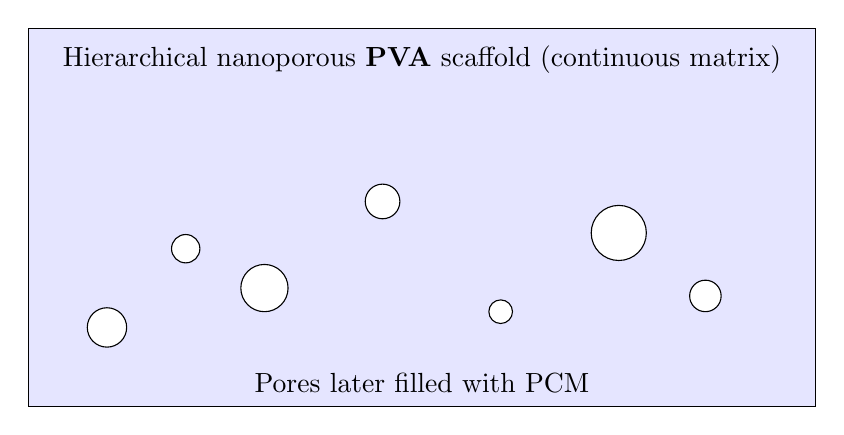
\begin{tikzpicture}
\draw[fill=blue!10] (0,0) rectangle (10,4.8);
\foreach \x/\y/\r in {1/1/0.25,2/2/0.18,3/1.5/0.30,4.5/2.6/0.22,6/1.2/0.15,7.5/2.2/0.35,8.6/1.4/0.2}{
\draw[fill=white] (\x,\y) circle (\r);
}
\node at (5,4.4) {Hierarchical nanoporous \textbf{PVA} scaffold (continuous matrix)};
\node at (5,0.3) {Pores later filled with PCM};
\end{tikzpicture}
\caption{Schematic pore hierarchy in a freeze-dried PVA scaffold.}
\label{fig:pva_hierarchy}
\end{figure}

\begin{table}[htbp]
\centering
\caption{Representative PVA scaffold design variables.}
\label{tab:pva_design}
\begin{tabular}{lcc}
\toprule
Variable & Symbol & Range \\
\midrule
Pore fraction & $\phi_p$ & 0.45--0.80 \\
Mean pore radius & $r_p$ & 100 nm--5 \si{\micro\meter} \\
Crystallinity index & $X_c$ & 0.25--0.55 \\
Crosslink density proxy & $\nu_x$ & 0.1--0.5 \\
\bottomrule
\end{tabular}
\end{table}

\begin{table}[htbp]
\centering
\caption{Mechanical cycling performance targets for PVA scaffold.}
\label{tab:pva_mech_targets}
\begin{tabular}{lcc}
\toprule
Metric & Target & Rationale \\
\midrule
Compression set after 1000 cycles & $<5\%$ & Maintain thermal contact \\
Strength retention $\sigma_f(N)/\sigma_f(0)$ & $>0.9$ & Structural reliability \\
Mass loss & $<1\%$ & PCM leakage control \\
\bottomrule
\end{tabular}
\end{table}
